\section{Conclusion}

In this report we have discussed the underlying theory, experimental procedure, results and analyzed the results with regard to the nature of the thiols and possible sources of errors.



\begin{figure}[h]
\centering
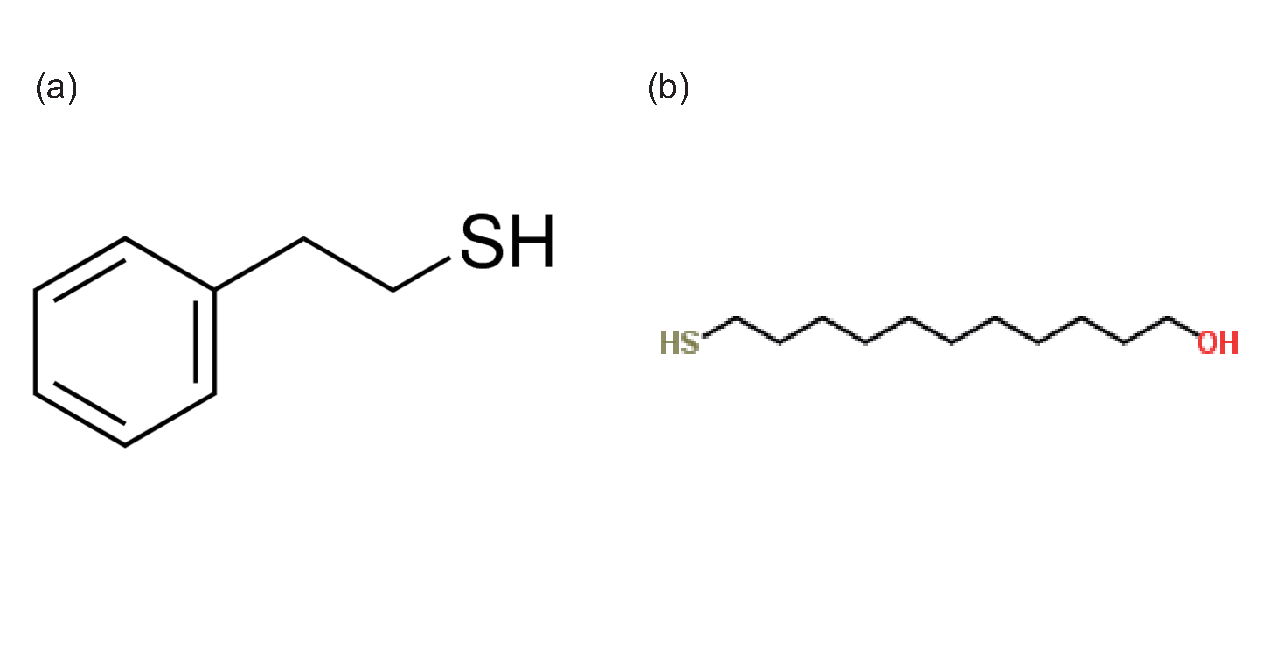
\includegraphics[width=0.9\columnwidth]{11mer.eps}
\caption{(a) The structure of 2-Phenylethanethiol. (b) The structure of 11-mercaptoundecanol. }
\label{11mer}
\end{figure}

We conclude our discussion on monolayers by giving a brief review of our findings on the topic of mixed monolayer stability in recent journal publications.
Yaliraki et al. presented a theoretical model for estimating monolayer stability based on concentrations and reaction temperature and present this in a series of computed phase diagrams. They tested these predictions and claim they could not co-assemble benzenethiols and alkanethiols on the same substrate. \cite{yaliraki}
Kang et al. presented results from a study on the properties of mixed monolayers prepared from differently substituted 4-mercaptobiphenyl on gold (1 1 1). They performed AFM and Infrared spectroscopy measurement on these monolayers. They found stabilities in excess of 1 month for the mixed monolayers. \cite{kang}
A review paper on the issues of self-assembled monolayers written by Srisombat et al. allocates a chapter to the issue of monolayers on flat gold surfaces. They review a wealth of papers hence I will focus on a couple of examples only. They give examples of findings which exhibited contact angle instability over time in mixed monolayers of an alkanethiol with non-polar termination and a polar hydroxyl terminated thiol. \cite{srisombat}
>>>>>>> Stashed changes
